\section{Navmesh (Bartosz Strzelecki)}

Komponent Unity Navmesh jest podstawowym elementem wykorzystywanym w przypadku znajdywania ścieżek.
Jest to mechanizm pozwalający na przechowywanie wyspecjalizowanych danych, które reprezentują
powierzchnie, po których mogą poruszać się agenty sztucznej inteligencji.

Aby zacząć korzystać z komponentu należy wygenerować mapę w edytorze Unity.
W ramach tego procesu wykonywane są obliczenia mające na celu wykrycie powierzchni,
po której może poruszać się dany agent. Ten system bierze pod uwagę kąt nachylenia
powierzchni, szerokość przejścia, jak i wysokość stropu.

W trakcie rozgrywki komponent NavMesh Agent wykorzystuje wcześniej wygenerowane dane
do wyznaczenia najlepszej ścieżki do celu. Z poziomu skryptów można dynamicznie modyfikować powierzchnię
nawigacyjną, umożliwiając w ten sposób uzyskanie poruszających się przeszkód i dynamicznie powstających budynków.

\begin{figure}[h!]
    \centering
    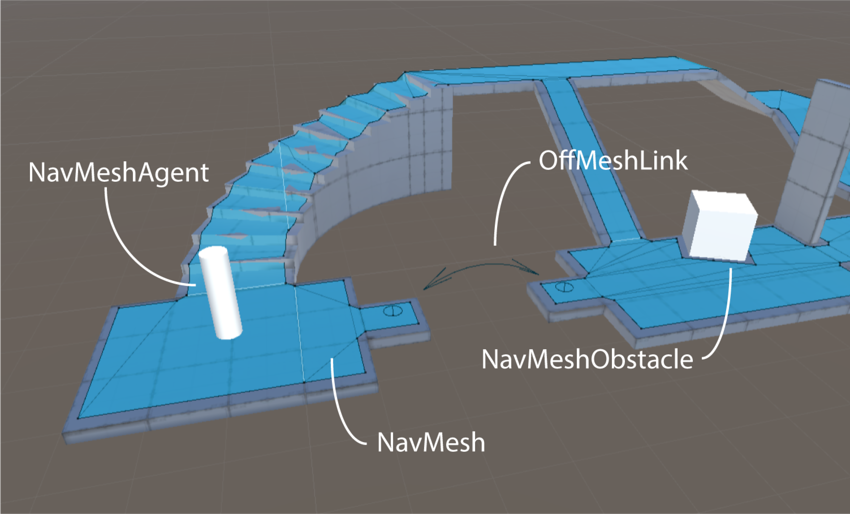
\includegraphics[width=0.9\textwidth]{images/navmesh.png}
    \caption{System nawigacji w Unity}
\end{figure}

Podsumowując system NavMesh istotnie upraszcza zadanie odnajdywania ścieżki, co pozwala na łatwe zaimplementowanie
realistycznych zachowań agentów sztucznej inteligencji. Znacznie ułatwia też zadanie tworzenia świata gry ze względu na automatyczny
sposób generowania danych nawigacyjnych.

